\documentclass{article}
\usepackage{graphicx}
\usepackage{amsmath}
\usepackage{hyperref}
\usepackage{siunitx}
\usepackage[super]{nth}
\usepackage{pgfplots}
\usepackage{filecontents}
\usepackage{listings}
\graphicspath{{../images/} }

%-------------------------------------------------------------------------------
%	TITLE SECTION
%-------------------------------------------------------------------------------

\newcommand{\horrule}[1]{\rule{\linewidth}{#1}} % Create horizontal rule command with 1 argument of height
\title{
\normalfont \normalsize
\textsc{Sapienza University of Rome} \\ [25pt]
\horrule{0.5pt} \\[0.4cm] % Thin top horizontal rule
\LARGE Planar Monocular SLAM \\
\large Probabilistic Robotics \\
\horrule{2pt} \\[0.5cm] % Thick bottom horizontal rule
}

\author{Ibis Prevedello}
\date{\normalsize\today}

\begin{document}
\maketitle

%-------------------------------------------------------------------------------
%	REPORT SECTION
%-------------------------------------------------------------------------------

\section{Introduction}
The goal of this project is to develop a SLAM system using Total Least Square algorithm to determine the trajectory of a robot moving in a given environment. This robot perceives the environment only using a stereo camera mounted on its base and its motion by the odometry sensor.

Before the optimization, the information known is the odometry for the trajectory and the landmarks position estimated by triangulation (first column of figure \ref{fig:landmark_and_pose} and the goal is to make the prediction match the ground truth values.

The program was written in Python and it succeeds in estimating the right trajectory of the robot and also most of the landmarks, with the exception of some that were bad initialized due to lack of information collected by the camera.

%-------------------------------------------------------------------------------

\section{Development}
First it is necessary to create a feature association, because the robot perceives the landmark appearance and do not know its id, it is necessary to determine what id each appearance corresponds to, matching with the descriptors of each landmark using l\textsuperscript{2}-norm.

Then, for the landmarks initialization, they need to be triangulated using Direct Linear Transformation (DLT) \cite{Hartley:2003:MVG:861369} for each landmark all the times that the robot perceived it. This process depends on the premise that the robot sees the landmark to know that it exists, it can also cause a bad accuracy triangulating its position if there is not enough information.

And finally, run the total least square algorithm with the pose-pose constraints give by the odometry and the pose-landmark constraints given the the images.

%-------------------------------------------------------------------------------
\section{Dataset}
The dataset for this project was generated using the \textbf{runba\_sim} simulator \cite{runba_sim} and is composed of four different class of files:

\subsection{camera.dat}
Information about the camera.
\begin{lstlisting}[mathescape=true]
CAMERA MATRIX
CAMERA TRANSFORMATION
Z NEAR
Z FAR
WIDTH
HEIGHT
\end{lstlisting}

\subsection{world.dat}
Information about the map.
\begin{lstlisting}[mathescape=true]
ID - X - Y - Z - APPEARANCE
\end{lstlisting}

\subsection{trajectory.dat}
Information about the trajectory of the robot, containing ground truth values and odometry values.
\begin{lstlisting}[mathescape=true]
POSE ID - GROUND TRUTH{X - Y - $\theta$} - ODOMETRY{X - Y - $\theta$}
\end{lstlisting}

\subsection{meas-xxxxx.dat}
Information about the data collected by the robot's camera, with image's position and appearance of each landmark.
\begin{lstlisting}[mathescape=true]
POSE ID
GROUND TRUTH{X - Y - $\theta$}
ODOMETRY{X - Y - $\theta$}
MEASUREMENT ID - LANDMARK GT ID - ROW - COLUMN - APPEARANCE
\end{lstlisting}

%-------------------------------------------------------------------------------
\section{Results}

The total least square algorithm runs in order to optimize the given constraints. This optimization ran for 28 iterations and it is possible to see the final result in image \ref{fig:landmark_and_pose}. On the bottom part of the image we can notice that the trajectory of the robot after optimization matches exactly the ground truth values.

\begin{figure}
  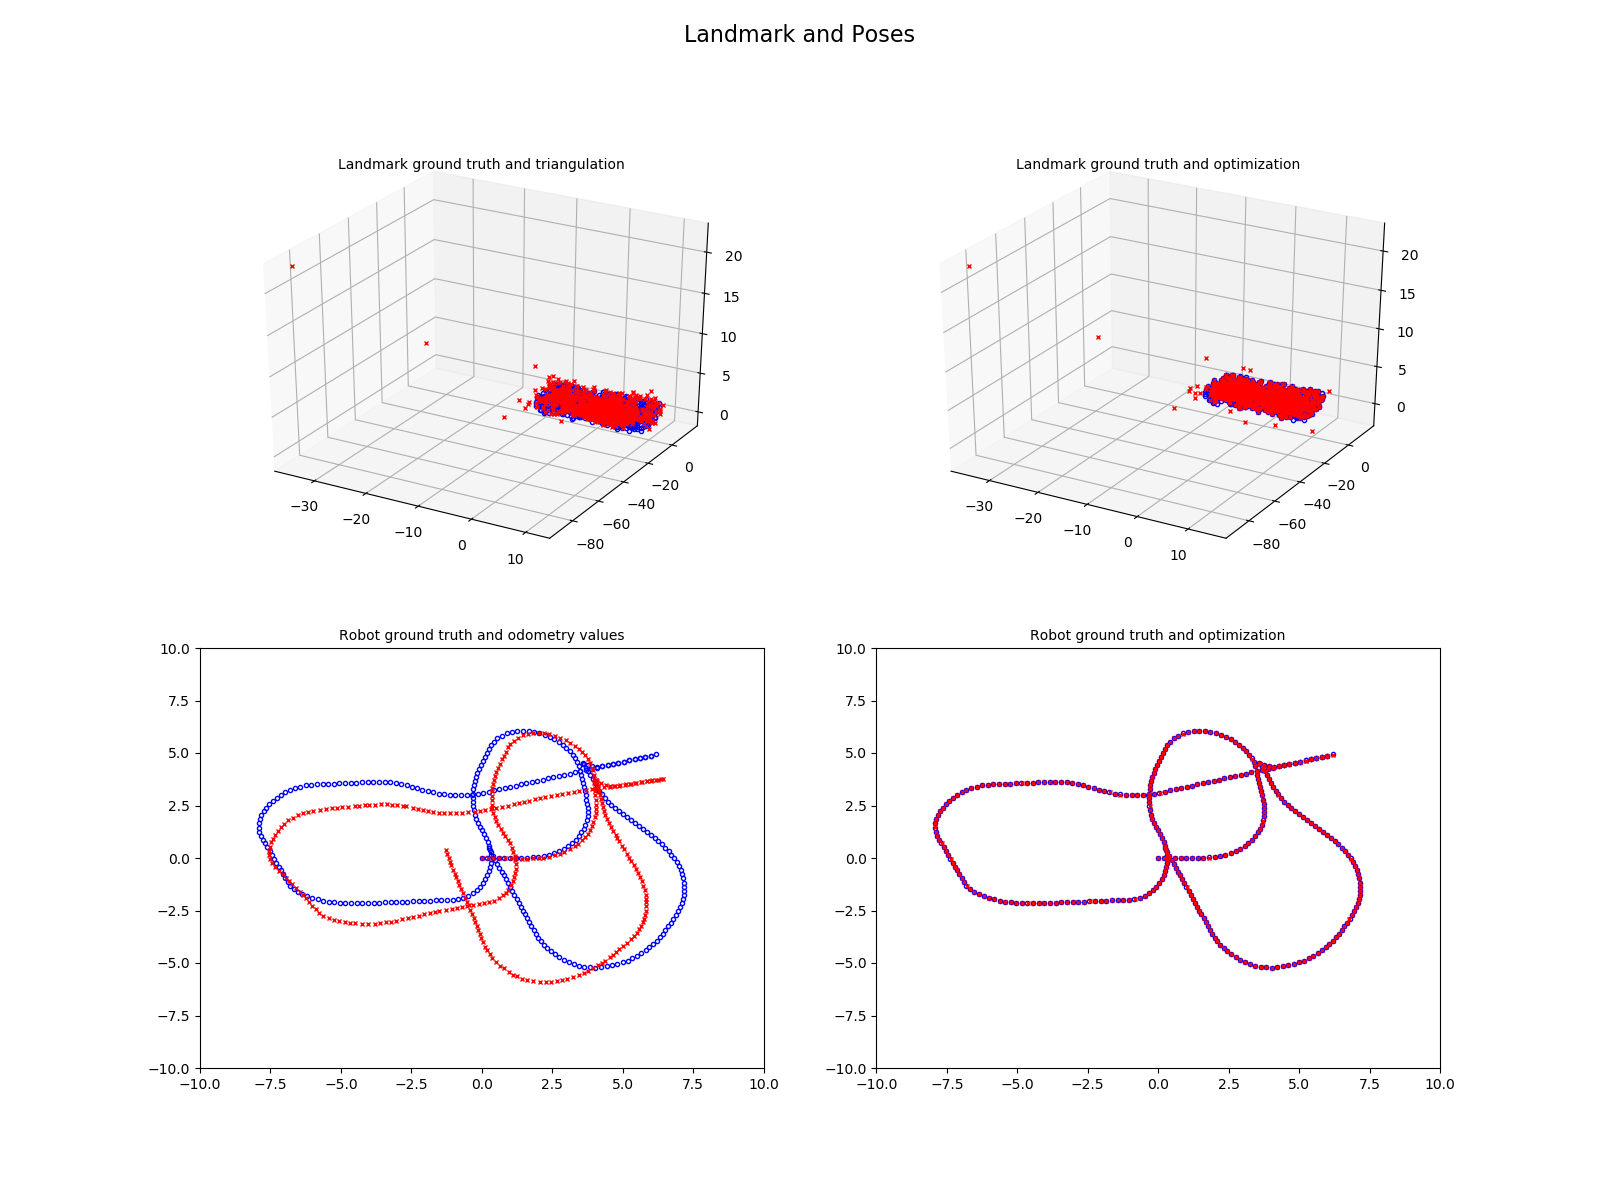
\includegraphics[scale=0.3]{landmark_and_pose.png}
  \centering
  \caption{Landmark and poses before and after optimization}
  \label{fig:landmark_and_pose}
\end{figure}

In image \ref{fig:landmark_and_pose} it is possible to notice some outliers landmarks badly initialized due to lack of information for the triangulation. In order to get a better view of the landmarks before and after optimization the outliers were removed and it can be seen in image \ref{fig:landmark_optimized}. From this image we can notice that most of the landmarks match the ground truth position after the optimization with the exception of some in the border of the world.

\begin{figure}
  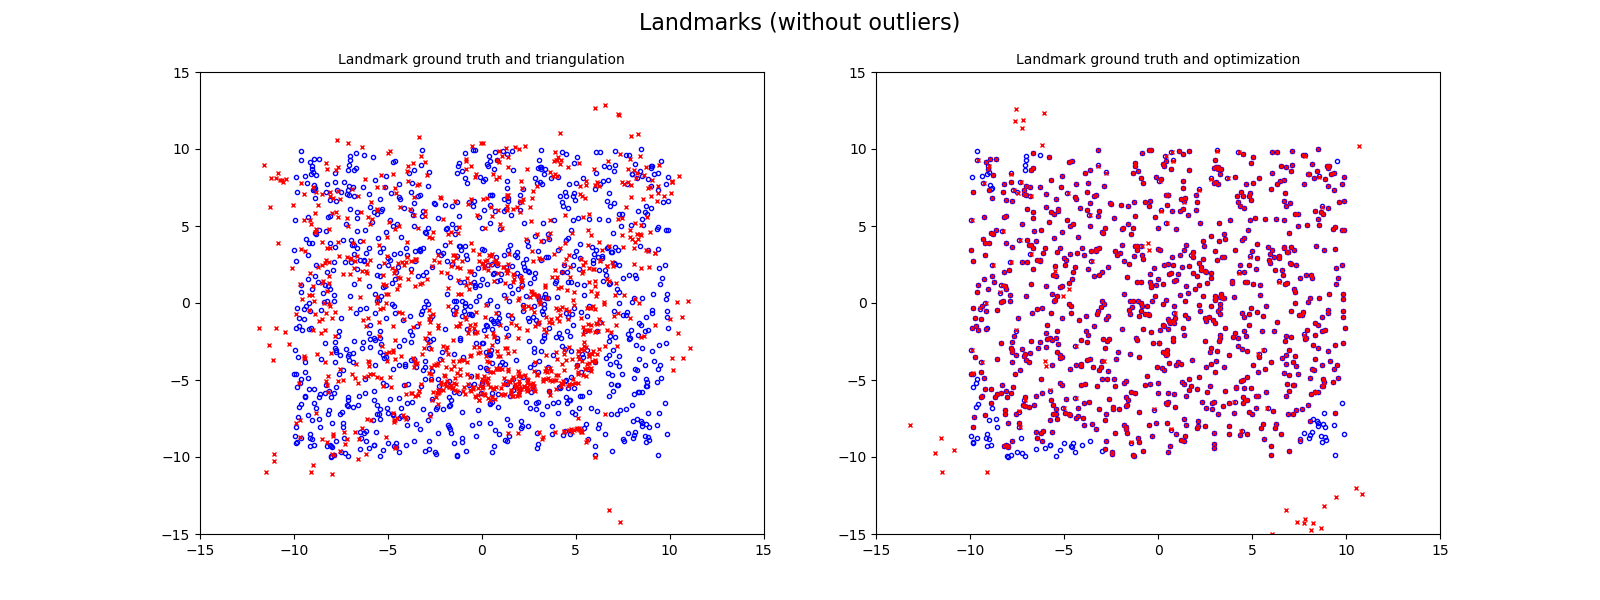
\includegraphics[scale=0.3]{landmarks_optimized.png}
  \centering
  \caption{Landmark before and after optimization}
  \label{fig:landmark_optimized}
\end{figure}

Image \ref{fig:chi_and_inliers} shows the chi and number of inliers for the poses and projections.

\begin{figure}
  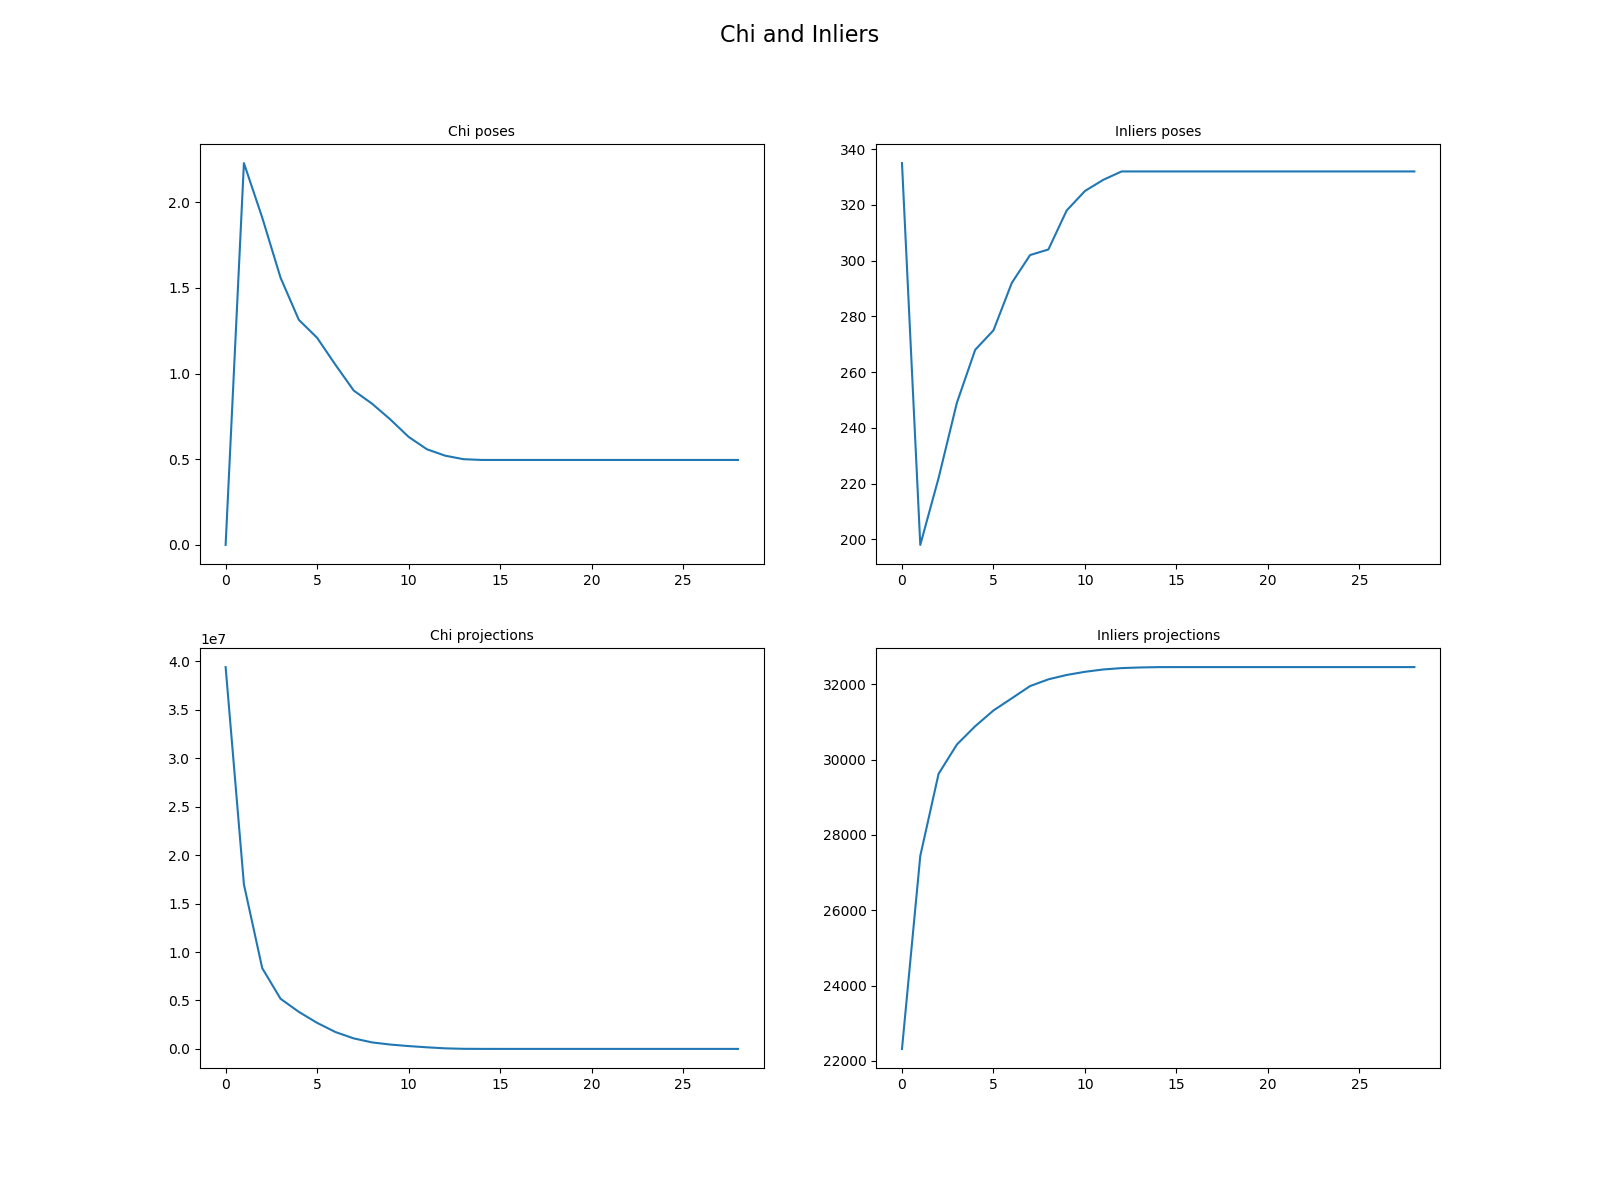
\includegraphics[scale=0.3]{chi_and_inliers.png}
  \centering
  \caption{Chi [left column] and inliers [right column] of the poses [first row] and the projections [second row] }
  \label{fig:chi_and_inliers}
\end{figure}

%-------------------------------------------------------------------------------

\section{Conclusion}

The algorithm implemented provided great results on trajectory and map optimization. Some of the landmarks that did not converge to the ground truth position were due to lack of information in the initialization, this could easily be solved with more data collected by the robot's camera.

This code was implemented in Python because the goal was just to understand how total least squares works, but another way to improve the performance of this algorithm would be converting the code to C++.


%-------------------------------------------------------------------------------
%	BIBLIOGRAPHY SECTION
%-------------------------------------------------------------------------------

\clearpage
\bibliography{bibliography}
\bibliographystyle{ieeetr}

%-------------------------------------------------------------------------------

\end{document}